
\includepdf[pages=2-3,scale=.8, nup=1x2, pagecommand=\subsection{Aufgaben}]{images/pdf/aufgabenfolien}

\includepdf[pages=4-,scale=.8, nup=1x2, pagecommand={}]{images/pdf/aufgabenfolien}


\subsubsection{Teilung der Aufgaben in Unteraufgaben zur Berechnung des Effektivitätsmaßes}

\begin{outline}[enumerate]
\newline
Aufgabe 1:\\
1. Karte mit richtiger Bezeichnung erstellen\\
2. Frist auf eine Woche festlegen\\
3. David assignen\\

\\Aufgabe 2:\\
4. Karte nach in Arbeit verschieben\\  
5. Erstes Item auf Checkliste abhaken\\
6. Zweites Item auf Checkliste abhaken\\

\\Aufgabe 3:\\
7. Eltern Karte archivieren\\  
8. Liste archivieren/löschen\\
9. Oma-Karte archivieren\\

\\Aufgabe 4:\\
10. Karte erstellen mit akkurater Bezeichnung\\
11. Checkliste erstellen\\
12. Checklist Items hinzufügen\\

\\Aufgabe 5:\\
13. Karte aus dem Archiv wiederherstellen\\
14. Karte in 'In Arbeit' verschieben\\
15. Farbliche Hervorhebung\\
\end{outline}

\begin{figure}[H]
    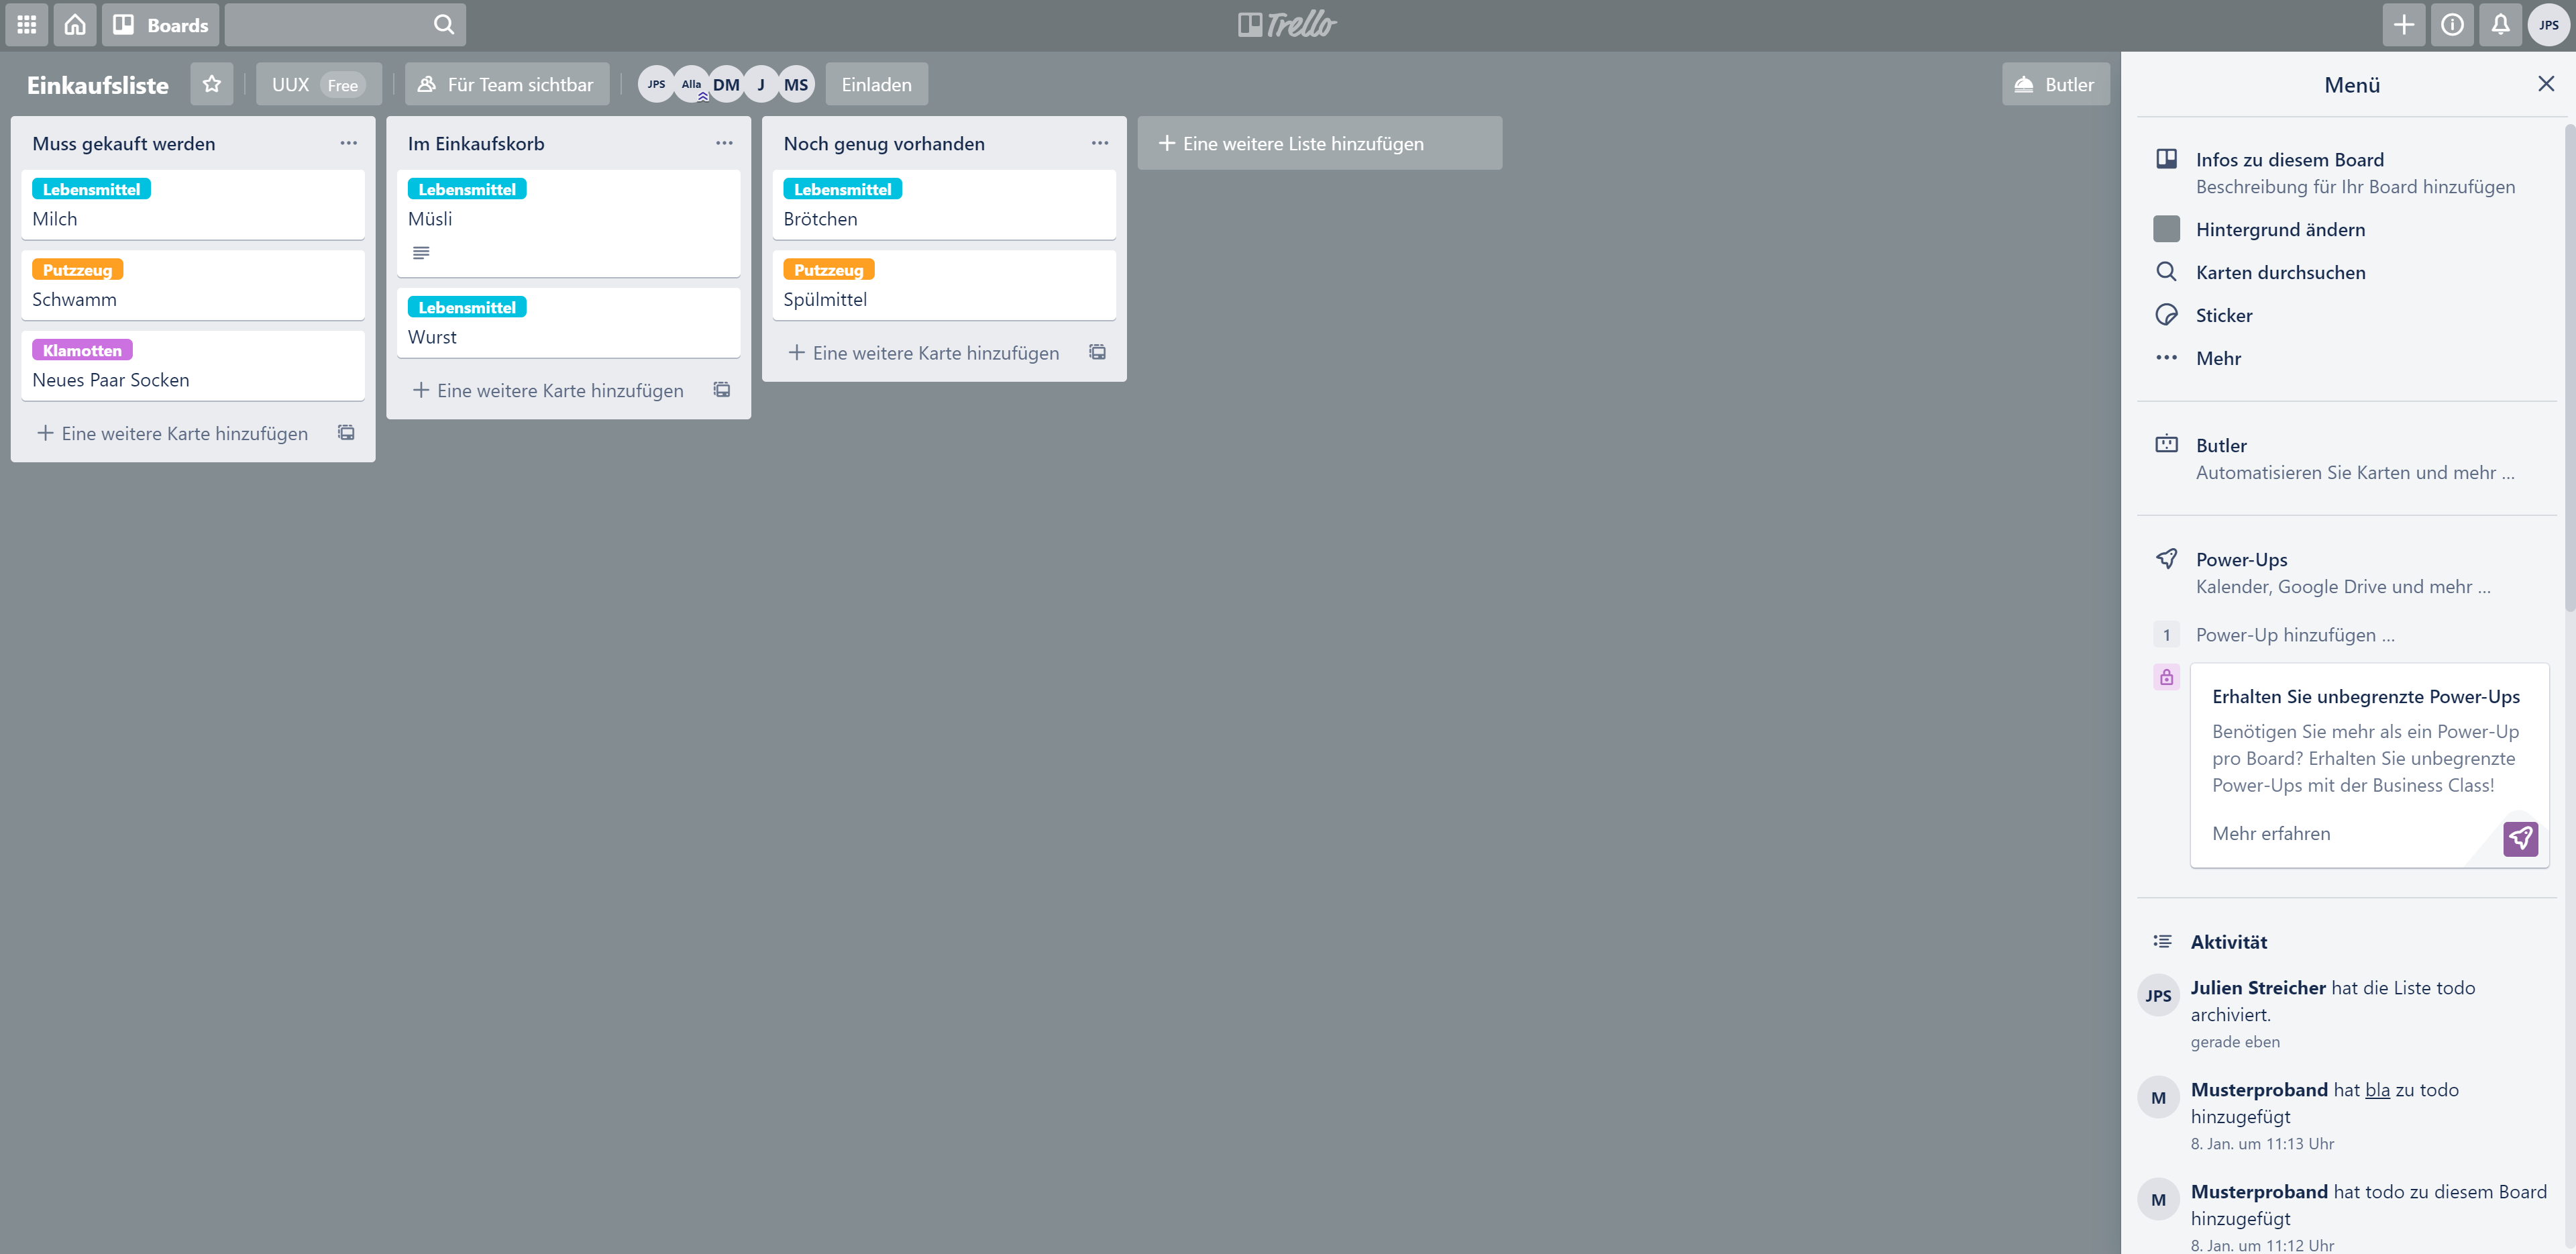
\includegraphics[width=\textwidth]{images/UI/Einkaufsliste.PNG}
    \centering
    \caption{Vorlagenboard 'Einkaufsliste' bei Trello}
    \label{fig:trelloeinkauf}
\end{figure}

\begin{figure}[H]
    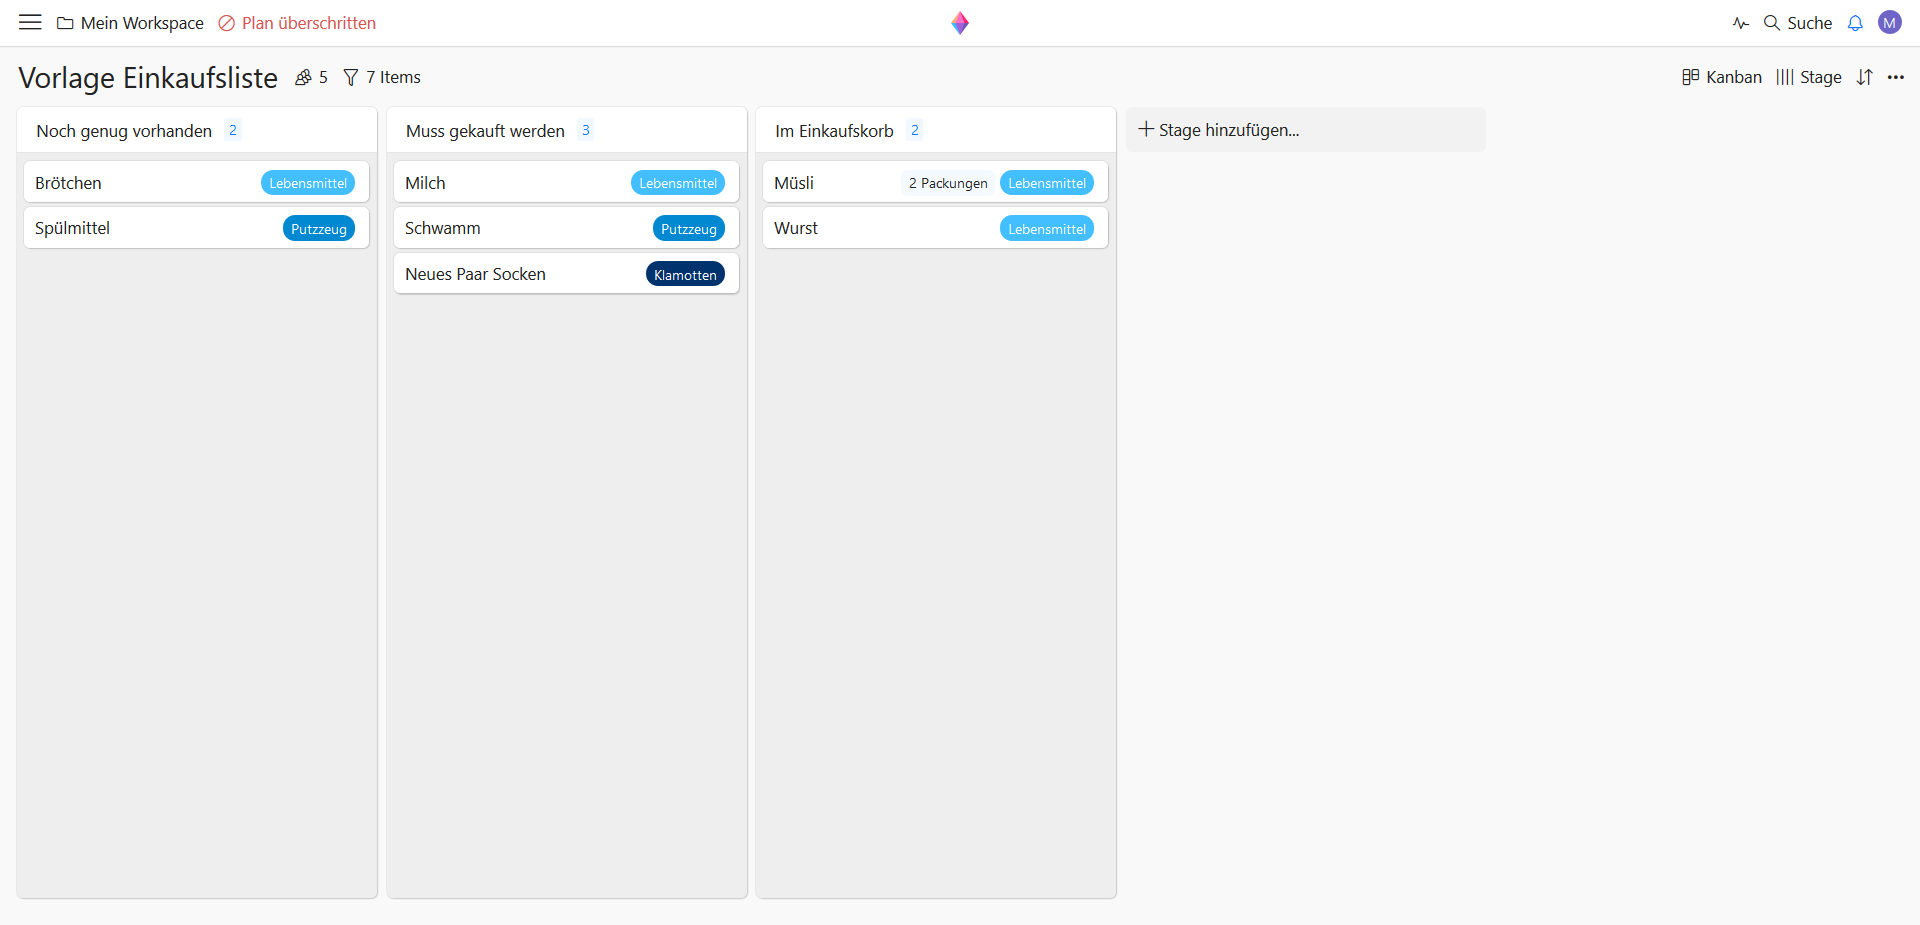
\includegraphics[width=\textwidth]{images/UI/zenkiteinkaufsliste.PNG}
    \centering
    \caption{Vorlagenboard 'Einkaufsliste' bei Zenkit}
    \label{fig:zenkiteinkauf}
\end{figure}

\begin{figure}[H]
    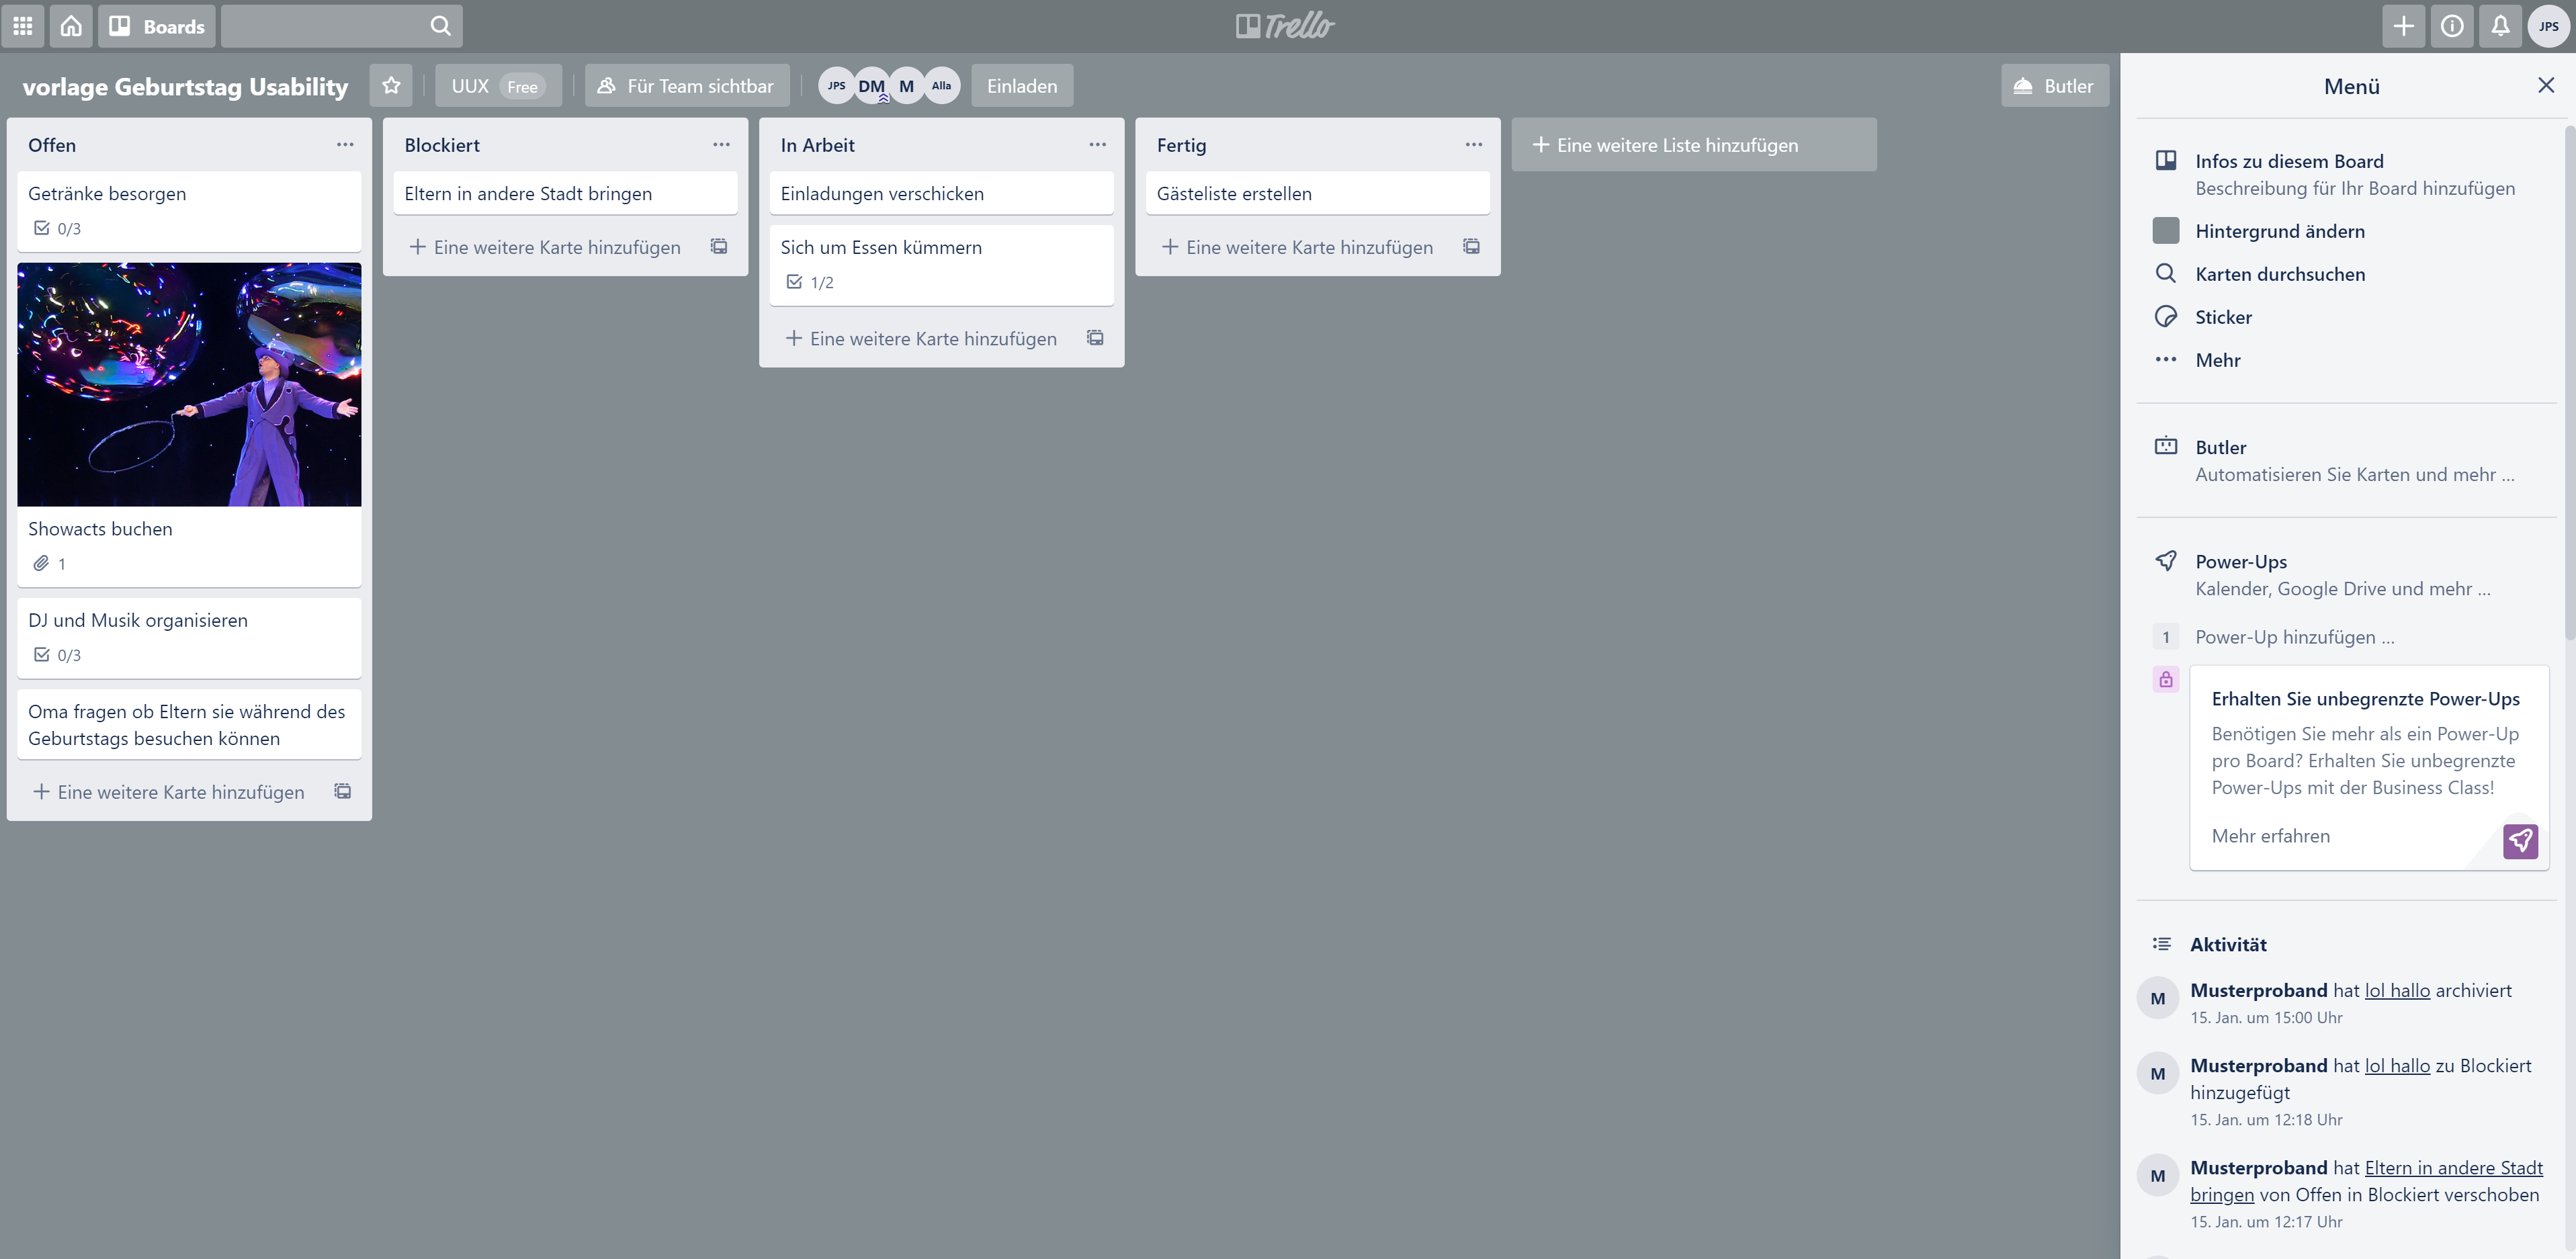
\includegraphics[width=\textwidth]{images/UI/Board Geburtstag.PNG}
    \centering
    \caption{Vorlagenboard 'Geburtstag' bei Trello}
    \label{fig:trellogebu}
\end{figure}

\begin{figure}[H]
    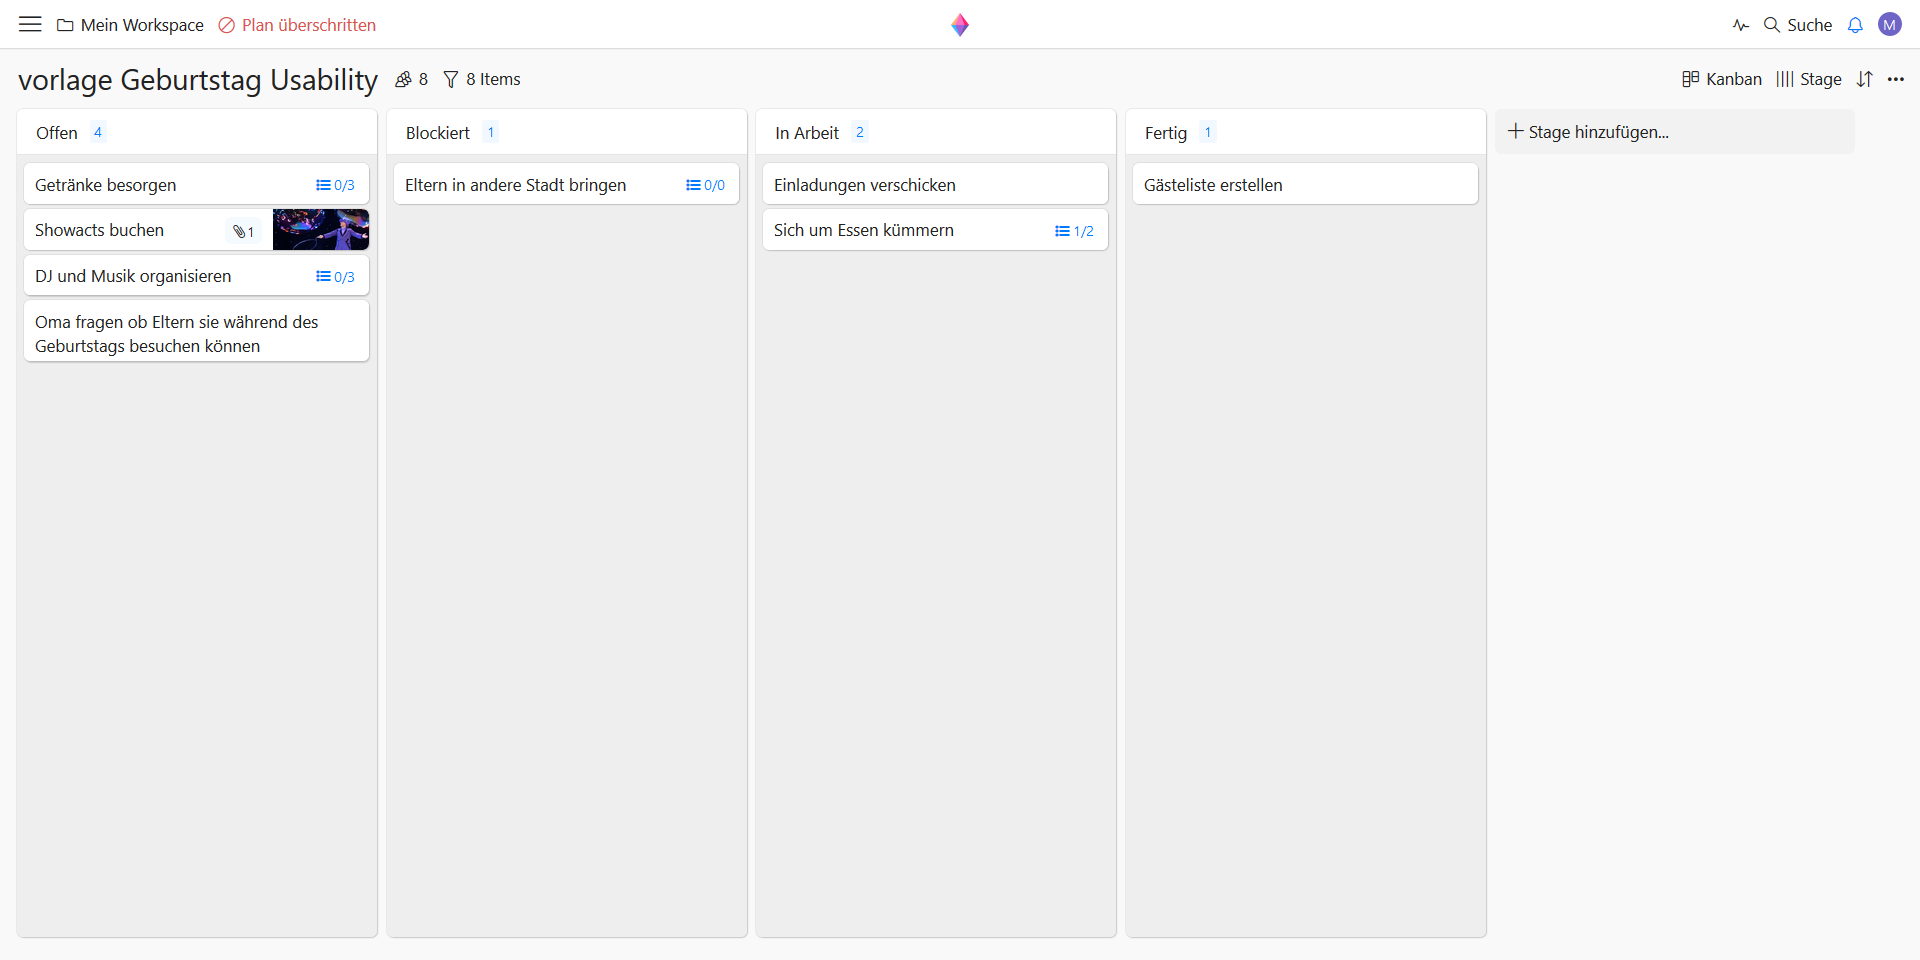
\includegraphics[width=\textwidth]{images/UI/geburtstagzenkit.PNG}
    \centering
    \caption{Vorlagenboard 'Geburtstag' bei Zenkit}
    \label{fig:zenkitgebu}
\end{figure}
